\section{Aim}
 To study string functions like, UPPER, LOWER, REVERSE, LPAD, LTRIM, RPAD, RTRIM, the LIKE keyword, and the wildcard characters.

\section{{Theory}}

\subsection{String Functions}
\begin{itemize}
	\item UPPER(str): Converts str to upper case.
	\item LOWER(str): Converts str to lower case.
	\item REVERSE(str): Reverses str.
	\item LPAD(str, len, padstr): Left pads the string to length len with the padding string padstr.
	\item RPAD(str, len, padstr): Right pads the string to length len with the padding string padstr.
	\item LTRIM(str, charset): Removes the characters from charset, from the left end of the string.
	\item RTRIM(str, charset): Removes the characters from charset, from the right end of the string.
	\item INITCAP(str): Changes the first letter of each word to its capital letter.
	\item CONCAT(str1, str2): Concatenates str2 to str1.
	\item LENGTH(str): Returns the length of the string str.
	\item SUBSTR(str, startindex, endindex): Returns the substring of str from startindex to endindex
\end{itemize}

\section{LIKE keyword}

The like keyword is used to match certain patterns in the strings. It is usually used in conjunction with two wildcard characters:
\begin{enumerate}
	\item \% character: This character matches zero or more occurances of any character\newline
	For example, 'A\%' can match any string starting with 'A'.
	\item \_ character: This character matches exactly one occurance of any character.\newline
	For example, 'A\_\_\_\_' matches any string starting with A, of length 5.
\end{enumerate}

\section{{Code and Output}}

\subsubsection{Create a table named acct\_details and populate the table as shown below.}

\newline
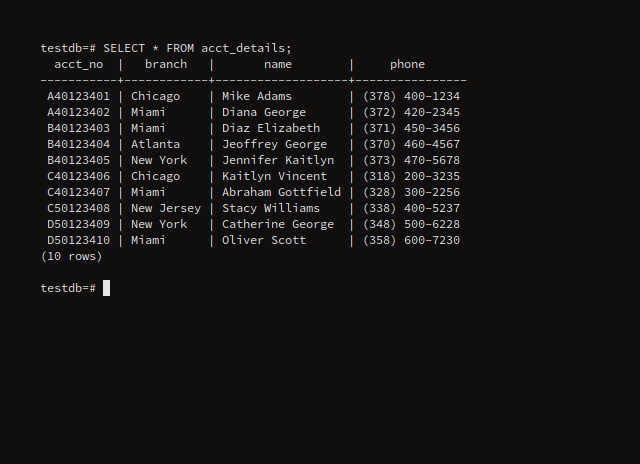
\includegraphics[width=\linewidth]{../Images/Strings/1.png}

\begin{enumerate}
\item Find the names of all people starting on the alphabet 'D'.\newline
\begin{minted}{sql}

SELECT name FROM acct_details WHERE name LIKE 'D%';

\end{minted}
\newline
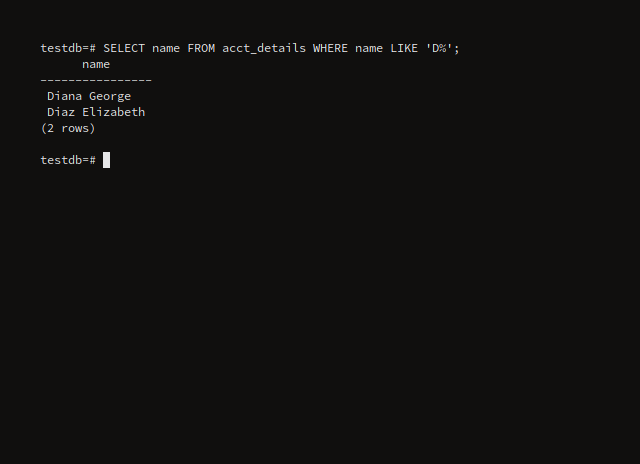
\includegraphics[width=\linewidth]{../Images/Strings/2.png}
\item List the names of all branches containing the substring 'New'.\newline
\begin{minted}{sql}

SELECT branch FROM acct_details WHERE branch LIKE '%New%';

\end{minted}
\newline
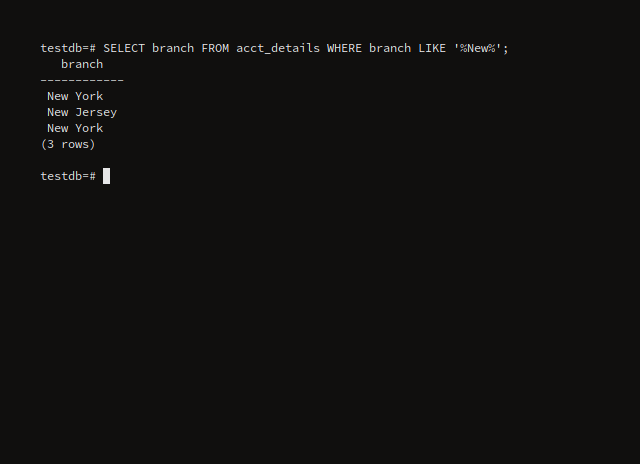
\includegraphics[width=\linewidth]{../Images/Strings/3.png}
\item List all the names in Upper Case Format.\newline
\begin{minted}{sql}

SELECT UPPER(name) FROM acct_details;

\end{minted}
\newline
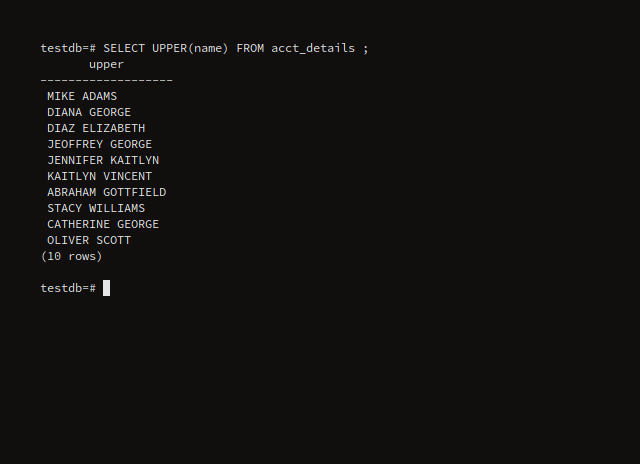
\includegraphics[width=\linewidth]{../Images/Strings/4.png}
\item List the names where the 4th letter is 'n' and last letter is 'n'.\newline
\begin{minted}{sql}

SELECT name FROM actt_details WHERE name LIKE '___n%n';

\end{minted}
\newline
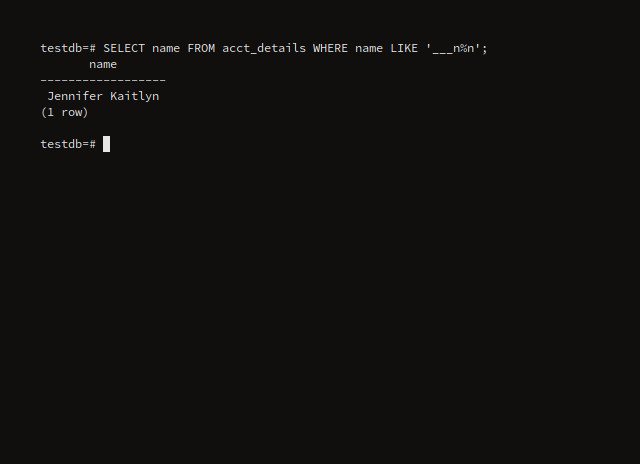
\includegraphics[width=\linewidth]{../Images/Strings/5.png}
\item List the names starting on 'D' , 3rd letter is 'a' and contains the substring 'Eli'.\newline
\begin{minted}{sql}

SELECT name FROM acct_details WHERE 
	name LIKE '%D_a%' AND LIKE '%Eli%';

\end{minted}
\newline
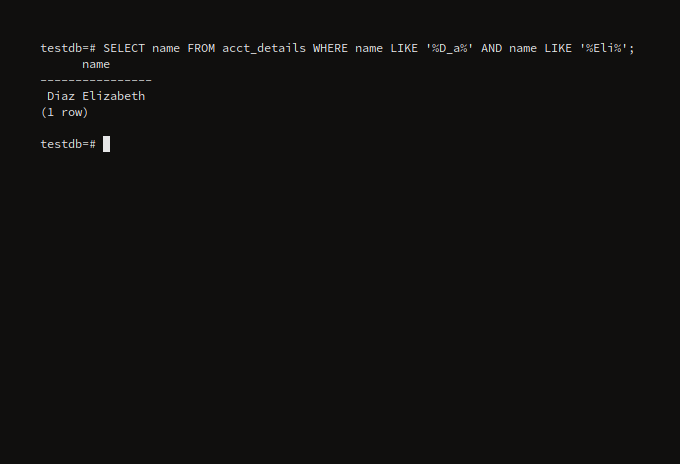
\includegraphics[width=\linewidth]{../Images/Strings/6.png}
\item List the names of people whose account number ends in '6'.\newline
\begin{minted}{sql}

SELECT name FROM acct_details WHERE acct_no LIKE '%6';

\end{minted}
\newline
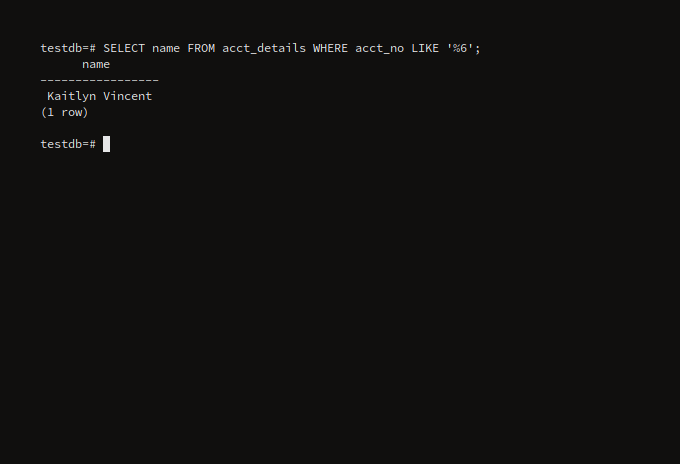
\includegraphics[width=\linewidth]{../Images/Strings/7.png}
\item Update the table so that all the names are in Upper Case Format.\newline
\begin{minted}{sql}

UPDATE acct_details SET name=UPPER(name);

\end{minted}
\newline
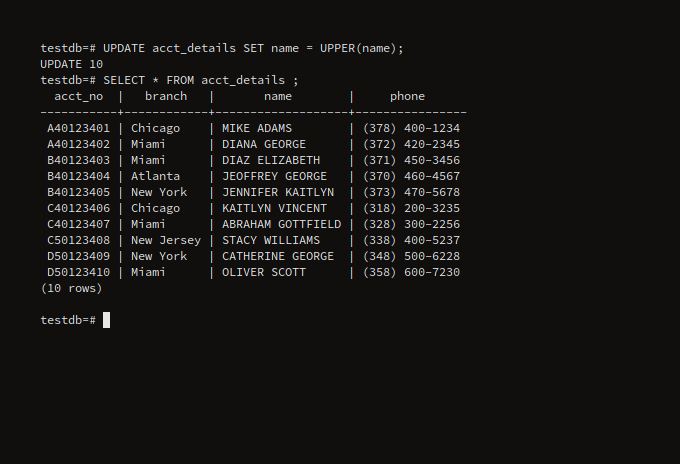
\includegraphics[width=\linewidth]{../Images/Strings/8.png}
\item List the names of all people ending on the alphabet 't'.\newline
\begin{minted}{sql}

SELECT name FROM acct_details WHERE name LIKE '%T';

\end{minted}
\newline
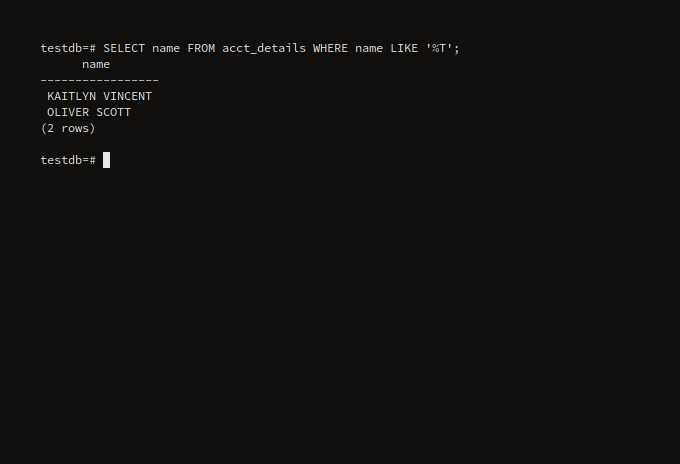
\includegraphics[width=\linewidth]{../Images/Strings/9.png}
\item List all the names in reverse.\newline
\begin{minted}{sql}

SELECT REVERSE(name) FROM acct_details;

\end{minted}
\newline
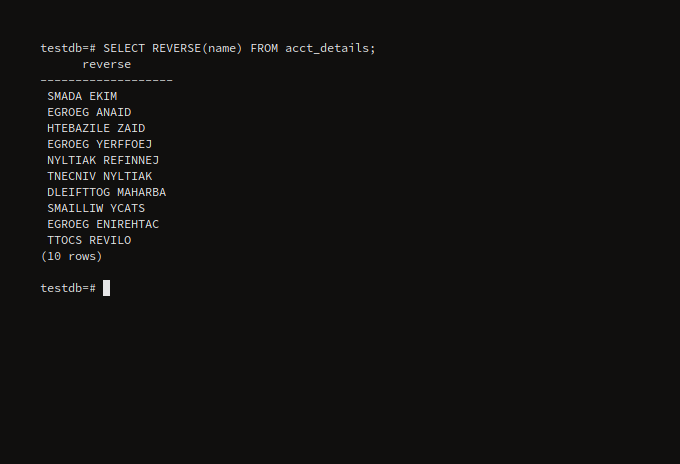
\includegraphics[width=\linewidth]{../Images/Strings/10.png}
\item Display all the phone numbers including US Country code ( +1). For eg: (378)400-1234 should be displayed as +1(378)400-1234. Use LPAD function.\newline
\begin{minted}{sql}

SELECT LPAD(phone, 16, '+1') FROM acct_details;

\end{minted}
\newline
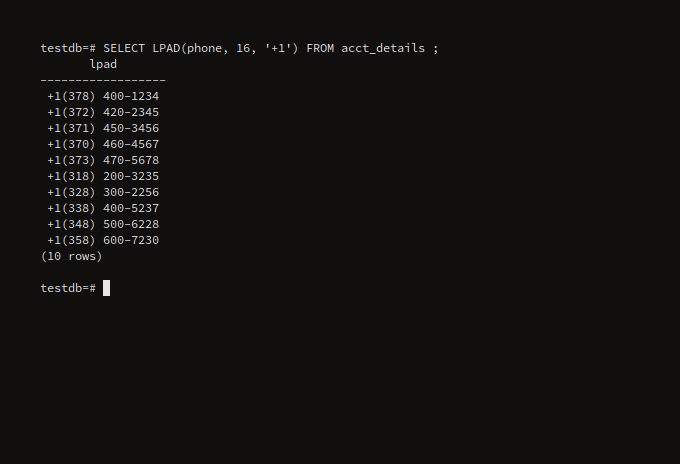
\includegraphics[width=\linewidth]{../Images/Strings/11.png}
\item Display all the account numbers. The starting alphabet associated with the Account\_No should be removed. Use LTRIM function.\newline
\begin{minted}{sql}

SELECT LTRIM(acct_no, '[ABCD]') AS acc_no, 
	branch, name, phone FROM acct_details;

\end{minted}
\newline
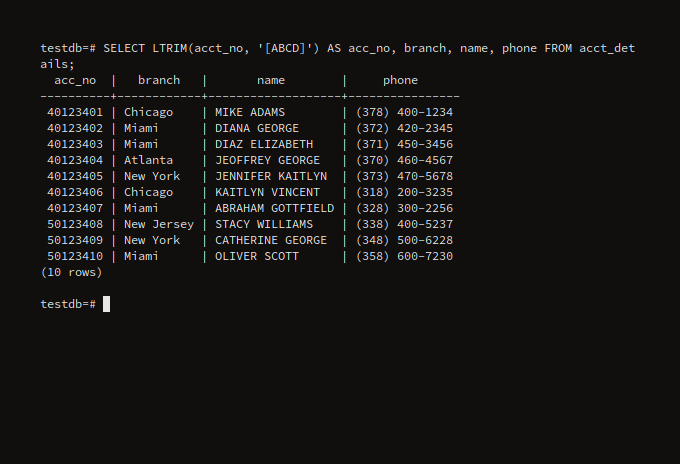
\includegraphics[width=\linewidth]{../Images/Strings/12.png}
\item Display the details of all people whose account number starts in '4' and name contains the substring 'Williams'.\newline
\begin{minted}{sql}

SELECT * FROM acct_details WHERE 
	acct_no LIKE '_4%' AND name LIKE '%WILLIAMS%';

SELECT * FROM acct_details WHERE 
	acct_no LIKE '_5%' AND name LIKE '%WILLIAMS%';

\end{minted}
\newline
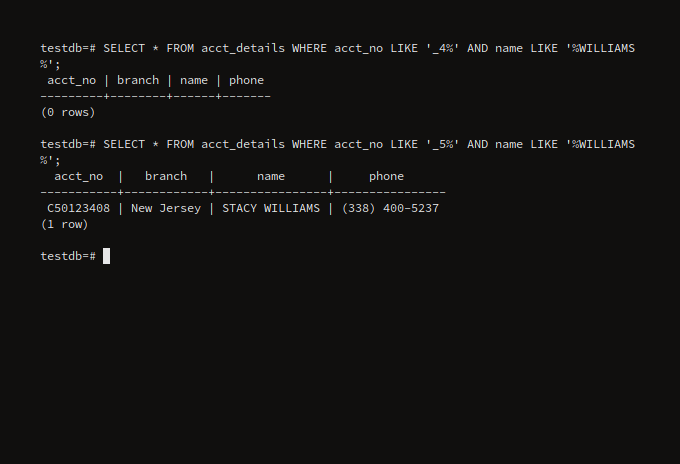
\includegraphics[width=\linewidth]{../Images/Strings/13.png}
\end{enumerate}

\subsubsection{String Functions}

\begin{enumerate}
\item Find the reverse of the string 'nmutuAotedOehT'.\newline
\begin{minted}{sql}

SELECT REVERSE('nmutuAotedOehT')

\end{minted}
\newline
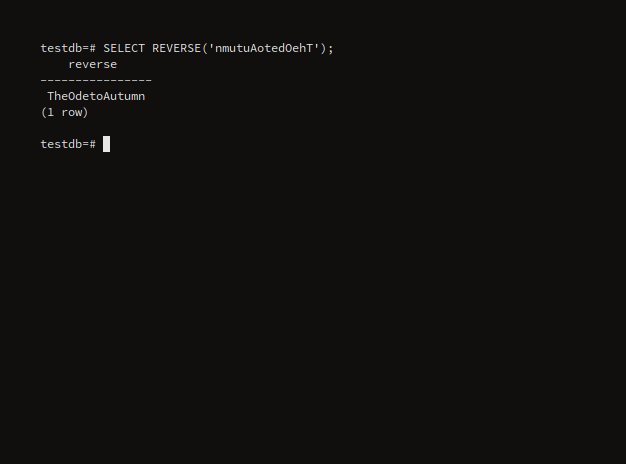
\includegraphics[width=\linewidth]{../Images/Strings/14.png}
\item Use LTRIM function on '123231xyzTech' so as to obtain the output 'Tech'.\newline
\begin{minted}{sql}

SELECT LTRIM('123231xyzTech', '123XYZ');

\end{minted}
\newline
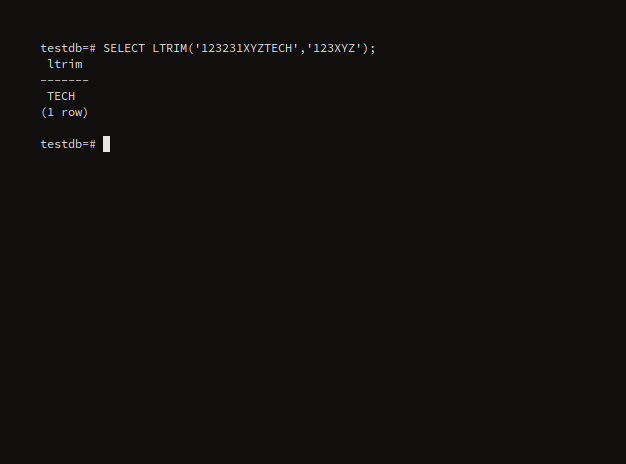
\includegraphics[width=\linewidth]{../Images/Strings/15.png}
\item Use RTRIM function on 'Computer ' to remove the trailing spaces.\newline
\begin{minted}{sql}

SELECT RTRIM('COMPUTER      ');

\end{minted}
\newline
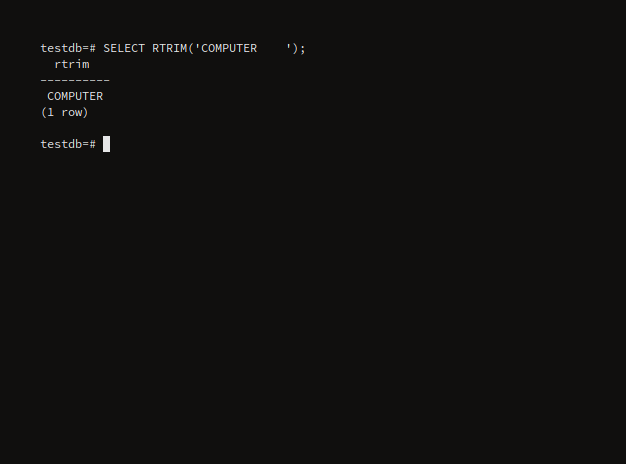
\includegraphics[width=\linewidth]{../Images/Strings/16.png}
\item Perform RPAD on 'computer' to obtain the output as 'computerXXXX'.\newline
\begin{minted}{sql}

SELECT RPAD('COMPUTER', 12, 'X');

\end{minted}
\newline
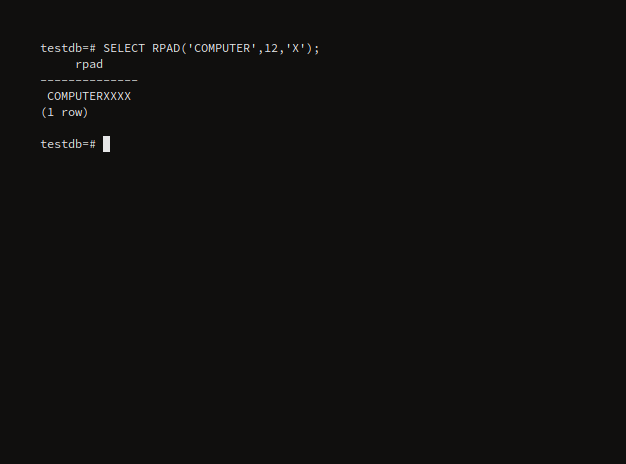
\includegraphics[width=\linewidth]{../Images/Strings/17.png}
\item Perform INITCAP function on 'mARK cALAwaY'.\newline
\begin{minted}{sql}

SELECT INITCAP('mARK cALAwaY')

\end{minted}
\newline
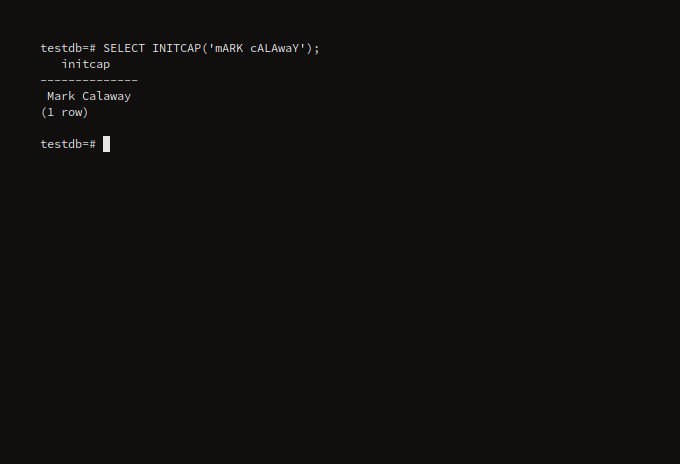
\includegraphics[width=\linewidth]{../Images/Strings/18.png}
\item Find the length of the string 'Database Management Systems'.\newline
\begin{minted}{sql}

SELECT LENGTH('Database Management Systems');

\end{minted}
\newline
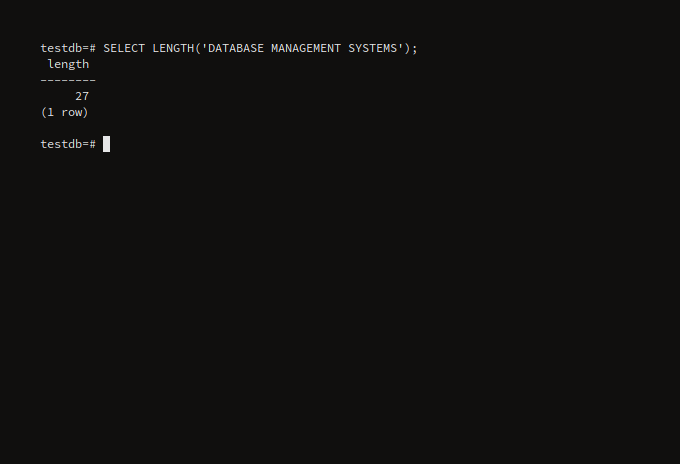
\includegraphics[width=\linewidth]{../Images/Strings/19.png}
\item Concatenate the strings 'Julius' and 'Caesar'\newline
\begin{minted}{sql}

SELECT CONCAT('Julius', 'Caesar');

\end{minted}
\newline
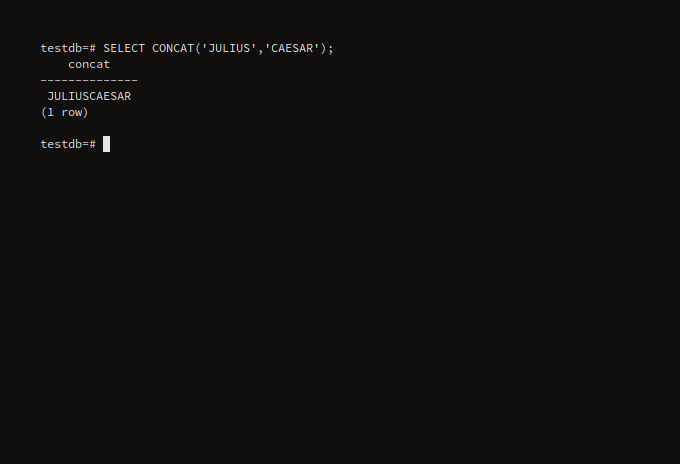
\includegraphics[width=\linewidth]{../Images/Strings/20.png}
\item Use SUBSTR function to retrieve the substring 'is' from the string 'India is my country'.\newline
\begin{minted}{sql}

SELECT SUBSTR('India is my country', 7, 2);

\end{minted}
\newline
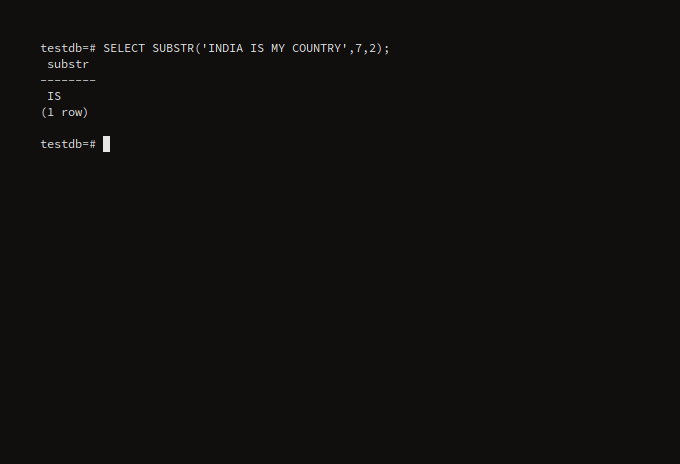
\includegraphics[width=\linewidth]{../Images/Strings/21.png}
\end{enumerate}

\section{Result}
Implemented the program for String Functions and Pattern Matching using Postgresql 11.5 on Manjaro Linux and the output was obtained.